
\documentclass[letterpaper,hide notes,xcolor={table,svgnames},pdftex,10pt]{beamer}
\def\showexamples{t}


%\usepackage[svgnames]{xcolor}

%% Demo talk
%\documentclass[letterpaper,notes=show]{beamer}

\usecolortheme{crane}
\setbeamertemplate{navigation symbols}{}

\usetheme{MyPittsburgh}
%\usetheme{Frankfurt}

%\usepackage{tipa}

\usepackage{hyperref}
\usepackage{graphicx,xspace}
\usepackage[normalem]{ulem}
\usepackage{multicol}
\usepackage{amsmath,amssymb,amsthm,graphicx,xspace}
\newcommand\SF[1]{$\bigstar$\footnote{SF: #1}}

\usepackage[default]{sourcesanspro}
\usepackage[T1]{fontenc}
\usepackage[scaled]{beramono}
\usepackage{tikzpagenodes}

\newcounter{tmpnumSlide}
\newcounter{tmpnumNote}


% old question code
%\newcommand\question[1]{{$\bigstar$ \small \onlySlide{2}{#1}}}
% \newcommand\nquestion[1]{\ifdefined \presentationonly \textcircled{?} \fi \note{\par{\Large \textbf{?}} #1}}
% \newcommand\nanswer[1]{\note{\par{\Large \textbf{A}} #1}}


 \newcommand\mnote[1]{%
   \addtocounter{tmpnumSlide}{1}
   \ifdefined\showcues {~\tiny\fbox{\arabic{tmpnumSlide}}}\fi
   \note{\setlength{\parskip}{1ex}\addtocounter{tmpnumNote}{1}\textbf{\Large \arabic{tmpnumNote}:} {#1\par}}}

\newcommand\mmnote[1]{\note{\setlength{\parskip}{1ex}#1\par}}

%\newcommand\mnote[2][]{\ifdefined\handoutwithnotes {~\tiny\fbox{#1}}\fi
% \note{\setlength{\parskip}{1ex}\textbf{\Large #1:} #2\par}}

%\newcommand\mnote[2][]{{\tiny\fbox{#1}} \note{\setlength{\parskip}{1ex}\textbf{\Large #1:} #2\par}}

\newcommand\mquestion[2]{{~\color{red}\fbox{?}}\note{\setlength{\parskip}{1ex}\par{\Large \textbf{?}} #1} \note{\setlength{\parskip}{1ex}\par{\Large \textbf{A}} #2\par}\ifdefined \presentationonly \pause \fi}

\newcommand\blackboard[1]{%
\ifdefined   \showblackboard
  {#1}
  \else {\begin{center} \fbox{\colorbox{blue!30}{%
         \begin{minipage}{.95\linewidth}%
           \hspace{\stretch{1}} Some space intentionally left blank; done at the blackboard.%
         \end{minipage}}}\end{center}}%
         \fi%
}



%\newcommand\q{\tikz \node[thick,color=black,shape=circle]{?};}
%\newcommand\q{\ifdefined \presentationonly \textcircled{?} \fi}

\usepackage{listings}
\lstset{basicstyle=\footnotesize\ttfamily,
	breaklines=true,
	aboveskip=15pt,
  	belowskip=15pt,
	frame=lines,
	numbers=left, basicstyle=\scriptsize, numberstyle=\tiny, stepnumber=0, numbersep=2pt
}

\usepackage{siunitx}
\newcommand\sius[1]{\num[group-separator = {,}]{#1}\si{\micro\second}}
\newcommand\sims[1]{\num[group-separator = {,}]{#1}\si{\milli\second}}
\newcommand\sins[1]{\num[group-separator = {,}]{#1}\si{\nano\second}}
\sisetup{group-separator = {,}, group-digits = true}

%% -------------------- tikz --------------------
\usepackage{tikz}
\usetikzlibrary{positioning}
\usetikzlibrary{arrows,backgrounds,automata,decorations.shapes,decorations.pathmorphing,decorations.markings,decorations.text,decorations.pathreplacing}

\tikzstyle{place}=[circle,draw=blue!50,fill=blue!20,thick, inner sep=0pt,minimum size=6mm]
\tikzstyle{transition}=[rectangle,draw=black!50,fill=black!20,thick, inner sep=0pt,minimum size=4mm]

\tikzstyle{block}=[rectangle,draw=black, thick, inner sep=5pt]
\tikzstyle{bullet}=[circle,draw=black, fill=black, thin, inner sep=2pt]

\tikzstyle{pre}=[<-,shorten <=1pt,>=stealth',semithick]
\tikzstyle{post}=[->,shorten >=1pt,>=stealth',semithick]
\tikzstyle{bi}=[<->,shorten >=1pt,shorten <=1pt, >=stealth',semithick]

\tikzstyle{mut}=[-,>=stealth',semithick]

\tikzstyle{treereset}=[dashed,->, shorten >=1pt,>=stealth',thin]

\usepackage{ifmtarg}
\usepackage{xifthen}
\makeatletter
% new counter to now which frame it is within the sequence
\newcounter{multiframecounter}
% initialize buffer for previously used frame title
\gdef\lastframetitle{\textit{undefined}}
% new environment for a multi-frame
\newenvironment{multiframe}[1][]{%
\ifthenelse{\isempty{#1}}{%
% if no frame title was set via optional parameter,
% only increase sequence counter by 1
\addtocounter{multiframecounter}{1}%
}{%
% new frame title has been provided, thus
% reset sequence counter to 1 and buffer frame title for later use
\setcounter{multiframecounter}{1}%
\gdef\lastframetitle{#1}%
}%
% start conventional frame environment and
% automatically set frame title followed by sequence counter
\begin{frame}%
\frametitle{\lastframetitle~{\normalfont(\arabic{multiframecounter})}}%
}{%
\end{frame}%
}
\makeatother

\makeatletter
\newdimen\tu@tmpa%
\newdimen\ydiffl%
\newdimen\xdiffl%
\newcommand\ydiff[2]{%
    \coordinate (tmpnamea) at (#1);%
    \coordinate (tmpnameb) at (#2);%
    \pgfextracty{\tu@tmpa}{\pgfpointanchor{tmpnamea}{center}}%
    \pgfextracty{\ydiffl}{\pgfpointanchor{tmpnameb}{center}}%
    \advance\ydiffl by -\tu@tmpa%
}
\newcommand\xdiff[2]{%
    \coordinate (tmpnamea) at (#1);%
    \coordinate (tmpnameb) at (#2);%
    \pgfextractx{\tu@tmpa}{\pgfpointanchor{tmpnamea}{center}}%
    \pgfextractx{\xdiffl}{\pgfpointanchor{tmpnameb}{center}}%
    \advance\xdiffl by -\tu@tmpa%
}
\makeatother
\newcommand{\copyrightbox}[3][r]{%
\begin{tikzpicture}%
\node[inner sep=0pt,minimum size=2em](ciimage){#2};
\usefont{OT1}{phv}{n}{n}\fontsize{4}{4}\selectfont
\ydiff{ciimage.south}{ciimage.north}
\xdiff{ciimage.west}{ciimage.east}
\ifthenelse{\equal{#1}{r}}{%
\node[inner sep=0pt,right=1ex of ciimage.south east,anchor=north west,rotate=90]%
{\raggedleft\color{black!50}\parbox{\the\ydiffl}{\raggedright{}#3}};%
}{%
\ifthenelse{\equal{#1}{l}}{%
\node[inner sep=0pt,right=1ex of ciimage.south west,anchor=south west,rotate=90]%
{\raggedleft\color{black!50}\parbox{\the\ydiffl}{\raggedright{}#3}};%
}{%
\node[inner sep=0pt,below=1ex of ciimage.south west,anchor=north west]%
{\raggedleft\color{black!50}\parbox{\the\xdiffl}{\raggedright{}#3}};%
}
}
\end{tikzpicture}
}


%% --------------------

%\usepackage[excludeor]{everyhook}
%\PushPreHook{par}{\setbox0=\lastbox\llap{MUH}}\box0}

%\vspace*{\stretch{1}

%\setbox0=\lastbox \llap{\textbullet\enskip}\box0}

\setlength{\parskip}{\fill}

\newcommand\noskips{\setlength{\parskip}{1ex}}
\newcommand\doskips{\setlength{\parskip}{\fill}}

\newcommand\xx{\par\vspace*{\stretch{1}}\par}
\newcommand\xxs{\par\vspace*{2ex}\par}
\newcommand\tuple[1]{\langle #1 \rangle}
\newcommand\code[1]{{\sf \footnotesize #1}}
\newcommand\ex[1]{\uline{Example:} \ifdefined \presentationonly \pause \fi
  \ifdefined\showexamples#1\xspace\else{\uline{\hspace*{2cm}}}\fi}

\newcommand\ceil[1]{\lceil #1 \rceil}


\AtBeginSection[]
{
   \begin{frame}
       \frametitle{Outline}
       \tableofcontents[currentsection]
   \end{frame}
}



\pgfdeclarelayer{edgelayer}
\pgfdeclarelayer{nodelayer}
\pgfsetlayers{edgelayer,nodelayer,main}

\tikzstyle{none}=[inner sep=0pt]
\tikzstyle{rn}=[circle,fill=Red,draw=Black,line width=0.8 pt]
\tikzstyle{gn}=[circle,fill=Lime,draw=Black,line width=0.8 pt]
\tikzstyle{yn}=[circle,fill=Yellow,draw=Black,line width=0.8 pt]
\tikzstyle{empty}=[circle,fill=White,draw=Black]
\tikzstyle{bw} = [rectangle, draw, fill=blue!20, 
    text width=4em, text centered, rounded corners, minimum height=2em]
    
    \newcommand{\CcNote}[1]{% longname
	This work is licensed under the \textit{Creative Commons #1 3.0 License}.%
}
\newcommand{\CcImageBy}[1]{%
	\includegraphics[scale=#1]{creative_commons/cc_by_30.pdf}%
}
\newcommand{\CcImageSa}[1]{%
	\includegraphics[scale=#1]{creative_commons/cc_sa_30.pdf}%
}
\newcommand{\CcImageNc}[1]{%
	\includegraphics[scale=#1]{creative_commons/cc_nc_30.pdf}%
}
\newcommand{\CcGroupBySa}[2]{% zoom, gap
	\CcImageBy{#1}\hspace*{#2}\CcImageNc{#1}\hspace*{#2}\CcImageSa{#1}%
}
\newcommand{\CcLongnameByNcSa}{Attribution-NonCommercial-ShareAlike}

\newenvironment{changemargin}[1]{% 
  \begin{list}{}{% 
    \setlength{\topsep}{0pt}% 
    \setlength{\leftmargin}{#1}% 
    \setlength{\rightmargin}{1em}
    \setlength{\listparindent}{\parindent}% 
    \setlength{\itemindent}{\parindent}% 
    \setlength{\parsep}{\parskip}% 
  }% 
  \item[]}{\end{list}} 




\title{Lecture 18 --- Reentrancy, Inlining, HLL }

\author{Patrick Lam \\ \small \texttt{patrick.lam@uwaterloo.ca}}
\institute{Department of Electrical and Computer Engineering \\
  University of Waterloo}
\date{\today}


\begin{document}

\begin{frame}
  \titlepage

 \end{frame}

%%%%%%%%%%%%%%%%%%%%%%%%%%%%%%%%%%%%%%%%%%%%%%%%%%%%%%%%%%%%%%%%%%%%%%%%%%%%%%%%

\part{Reentrancy}
\frame{\partpage}

\begin{frame}[fragile]
\frametitle{Non-Reentrant C Function}

The trivial example of a non-reentrant C function:

\begin{lstlisting}[language=C]
int tmp;

void swap( int x, int y ) {
    tmp = y;
    y = x;
    x = tmp;
}
\end{lstlisting}

Why is this non-reentrant?

How can we make it reentrant?

\end{frame}

%%%%%%%%%%%%%%%%%%%%%%%%%%%%%%%%%%%%%%%%%%%%%%%%%%%%%%%%%%%%%%%%%%%%%%%%%%%%%%%%
\begin{frame}
  \frametitle{Reentrancy}

  
    $\Rightarrow$ A function can be suspended in the middle and \\ {\bf re-entered}
      (called again) before the previous execution returns.\\[1em]
    
     Does not always mean {\bf thread-safe} (although it usually is).
      \begin{itemize}
        \item Recall: {\bf thread-safe} is essentially ``no data races''.
      \end{itemize}
 ~\\[1em]
  Moot point if the function only modifies local data, e.g. {\tt sin()}.
  
\end{frame}
%%%%%%%%%%%%%%%%%%%%%%%%%%%%%%%%%%%%%%%%%%%%%%%%%%%%%%%%%%%%%%%%%%%%%%%%%%%%%%%%

%%%%%%%%%%%%%%%%%%%%%%%%%%%%%%%%%%%%%%%%%%%%%%%%%%%%%%%%%%%%%%%%%%%%%%%%%%%%%%%%
\begin{frame}[fragile]
  \frametitle{Reentrancy Example}

  

  Courtesy of Wikipedia (with modifications):
  \begin{lstlisting}[language=C]
int t;
 
void swap(int *x, int *y) {
    t = *x;
    *x = *y;
    // hardware interrupt might invoke isr() here!
    *y = t;
}
 
void isr() {
    int x = 1, y = 2;
    swap(&x, &y);
}
...
int a = 3, b = 4;
...
    swap(&a, &b);
  \end{lstlisting}
  
\end{frame}
%%%%%%%%%%%%%%%%%%%%%%%%%%%%%%%%%%%%%%%%%%%%%%%%%%%%%%%%%%%%%%%%%%%%%%%%%%%%%%%%

%%%%%%%%%%%%%%%%%%%%%%%%%%%%%%%%%%%%%%%%%%%%%%%%%%%%%%%%%%%%%%%%%%%%%%%%%%%%%%%%
\begin{frame}[fragile]
  \frametitle{Reentrancy Example---Explained (a trace)}

  
  \begin{lstlisting}[language=C]
call swap(&a, &b);
 t = *x;                // t = 3 (a)
 *x = *y;               // a = 4 (b)
 call isr();
    x = 1; y = 2;
    call swap(&x, &y)
    t = *x;             // t = 1 (x)
    *x = *y;            // x = 2 (y)
    *y = t;             // y = 1
 *y = t;                // b = 1

Final values:
a = 4, b = 1

Expected values:
a = 4, b = 3
  \end{lstlisting}
  
\end{frame}
%%%%%%%%%%%%%%%%%%%%%%%%%%%%%%%%%%%%%%%%%%%%%%%%%%%%%%%%%%%%%%%%%%%%%%%%%%%%%%%%

%%%%%%%%%%%%%%%%%%%%%%%%%%%%%%%%%%%%%%%%%%%%%%%%%%%%%%%%%%%%%%%%%%%%%%%%%%%%%%%%
\begin{frame}[fragile]
  \frametitle{Reentrancy Example, Fixed}

  
  \begin{lstlisting}[language=C][escapechar=@]
int t;
 
void swap(int *x, int *y) {
    int s;
 
    @\alert{s = t}@;  // save global variable
    t = *x;
    *x = *y;
    // hardware interrupt might invoke isr() here!
    *y = t;
    @\alert{t = s}@;  // restore global variable
}
 
void isr() {
    int x = 1, y = 2;
    swap(&x, &y);
}
...
int a = 3, b = 4;
...
    swap(&a, &b);
  \end{lstlisting}
  
\end{frame}
%%%%%%%%%%%%%%%%%%%%%%%%%%%%%%%%%%%%%%%%%%%%%%%%%%%%%%%%%%%%%%%%%%%%%%%%%%%%%%%%

%%%%%%%%%%%%%%%%%%%%%%%%%%%%%%%%%%%%%%%%%%%%%%%%%%%%%%%%%%%%%%%%%%%%%%%%%%%%%%%%
\begin{frame}[fragile]
  \frametitle{Reentrancy Example, Fixed---Explained (a trace)}

  
  \begin{lstlisting}[language=C]
call swap(&a, &b);
s = t;                 // s = UNDEFINED
t = *x;                // t = 3 (a)
*x = *y;               // a = 4 (b)
call isr();
    x = 1; y = 2;
    call swap(&x, &y)
    s = t;             // s = 3
    t = *x;            // t = 1 (x)
    *x = *y;           // x = 2 (y)
    *y = t;            // y = 1
    t = s;             // t = 3
*y = t;                // b = 3
t = s;                 // t = UNDEFINED

Final values:
a = 4, b = 3

Expected values:
a = 4, b = 3
  \end{lstlisting}
  
\end{frame}
%%%%%%%%%%%%%%%%%%%%%%%%%%%%%%%%%%%%%%%%%%%%%%%%%%%%%%%%%%%%%%%%%%%%%%%%%%%%%%%%

\begin{frame}
\frametitle{Interrupt Handling}


Remember that in things like interrupt subroutines (ISRs) having the code be reentrant is very important. 

Interrupts can get interrupted by higher priority interrupts and when that happens the ISR may simply be restarted, or we pause and resume.

Either way, if the code is not reentrant we will run into problems.


\end{frame}

\begin{frame}
\frametitle{Thread Safe vs. Reentrant}

Let us also draw a distinction between thread safe code and reentrant code. 

A thread safe operation is one that can be performed from more than one thread at the same time. 

On the other hand, a reentrant operation can be invoked while the operation is already in progress, possibly from within the same thread. 

Or it can be re-started without affecting the outcome. 

If a function is not reentrant, it may not be possible to make it thread safe. 

And furthermore, a reentrant function cannot call a non-reentrant one (and maintain its status as reentrant).

\end{frame}



\begin{frame}[fragile]
\frametitle{Thread Safe Non-Reentrant Example}
{\scriptsize
\begin{lstlisting}[language=C]
int length = 0;
char *s = NULL;

// Note: Since strings end with a 0, if we want to
// add a 0, we encode it as "\0", and encode a
// backslash as "\\".


// WARNING! This code is buggy - do not use!
void AddToString(int ch)
{
  EnterCriticalSection(&someCriticalSection);
  // +1 for the character we're about to add
  // +1 for the null terminator
  char *newString = realloc(s, (length+1) * sizeof(char));
  if (newString) {
    if (ch == '\0' || ch == '\\') {
      AddToString('\\'); // escape prefix
    }
    newString[length++] = ch;
    newString[length] = '\0';
    s = newString;
  }
  LeaveCriticalSection(&someCriticalSection);
}
\end{lstlisting}
}


\end{frame}



\begin{frame}
\frametitle{Analysis of This Example}

Is it thread safe? Sure---there is a critical section protected by the mutex \texttt{someCriticalSection}. 

But is is re-entrant? Nope. 

The internal call to \texttt{AddToString} causes a problem because the attempt to use \texttt{realloc} will use a pointer to \texttt{s}.

That is no longer valid because it got stomped by the earlier call to \texttt{realloc}.


\end{frame}



\begin{frame}
\frametitle{Functional Programming}

Interestingly, functional programming languages (NOT procedural like C) such as Scala and so on, lend themselves very nicely to being parallelized. 

Why? 

Because a purely functional program has no side effects and they are very easy to parallelize.

Any impure function has to indicate that in its function signature.

\end{frame}



\begin{frame}
\frametitle{Functional Programming}

\begin{center}
	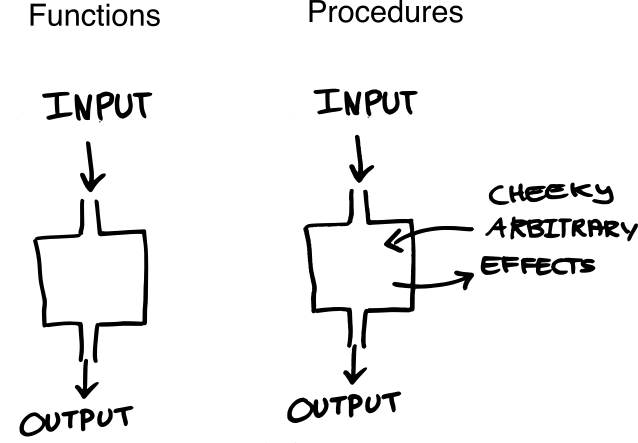
\includegraphics[width=0.8\textwidth]{images/functional.png}
\end{center}
{\small \url{https://www.fpcomplete.com/blog/2017/04/pure-functional-programming}}


\end{frame}



\begin{frame}
\frametitle{Joel on Functional}

\begin{quote}
\textit{Without understanding functional programming, you can't invent MapReduce, the algorithm that makes Google so massively scalable. The terms Map and Reduce come from Lisp and functional programming. MapReduce is, in retrospect, obvious to anyone who remembers from their 6.001-equivalent programming class that purely functional programs have no side effects and are thus trivially parallelizable.}
\end{quote}
\hfill --- Joel Spolsky


\end{frame}

\begin{frame}
\frametitle{OOP: \texttt{getBrain().damage()}}

Object oriented programming kind of gives us some bad habits in this regard. 

We tend to make a lot of \texttt{void} methods. 

In functional programming these don't really make sense, because if it's purely functional, then there are some inputs and some outputs. 

If a function returns nothing, what does it do? 

For the most part it can only have side effects which we would generally prefer to avoid if we can, if the goal is to parallelize things. 

\end{frame}

\begin{frame}
\frametitle{Functional Programming in Your C++}

{\tt algorithms} has been part of C++ since C++11.\\

C++17 (not well supported yet) introduces parallel and vectorized {\tt algorithms};\\
\qquad you specify an execution policy, compiler does it:\\
\qquad ({\tt sequenced}, {\tt parallel},
or {\tt parallel\_unsequenced}).\\[1em]

Some examples of algorithms:\\
\qquad {\tt sort}, {\tt reverse}, {\tt is\_heap}\ldots\\[1em]

Other examples of algorithms:\\
\qquad {\tt for\_each\_n}, {\tt exclusive\_scan}, {\tt reduce}\\[1em]
If you know functional programming (e.g. Haskell), these are:\\
\qquad {\tt map}, {\tt scanl}, {\tt fold1/foldl1}.

\end{frame}

\begin{frame}
\frametitle{Side Effects}

Side effects are sort of undesirable (and definitely not functional), but not necessarily bad. 

Printing to console is unavoidably making use of a side effect, but it's what we want. 

We don't want to call print reentrantly, because two threads trying to write at the same time to the console would result in jumbled output. 

Or alternatively, restarting the print routine might result in some doubled characters on the screen.

\end{frame}

\begin{frame}
\frametitle{Purity}

The notion of purity is related to side effects.

A function is \emph{pure} if it has no side effects and if its outputs depend solely on its inputs.

Pure functions should be implemented as thread-safe and reentrant.

\end{frame}







%%%%%%%%%%%%%%%%%%%%%%%%%%%%%%%%%%%%%%%%%%%%%%%%%%%%%%%%%%%%%%%%%%%%%%%%%%%%%%%%
\begin{frame}[fragile]
  \frametitle{Previous Example: thread-safety}

  
  Is the previous reentrant code also thread-safe?\\

  (This is more what we're concerned about in this course.)\\[1em]

  Let's see:
  \begin{lstlisting}[language=C]
int t;

void swap(int *x, int *y) {
    int s;
 
    s = t;  // save global variable
    t = *x;
    *x = *y;
    // hardware interrupt might invoke isr() here!
    *y = t;
    t = s;  // restore global variable
}
  \end{lstlisting}
  
  Consider two calls: {\tt swap(a, b)}, {\tt swap(c, d)} with\\
  \quad {\tt a = 1, b = 2, c = 3, d = 4}.
  
\end{frame}
%%%%%%%%%%%%%%%%%%%%%%%%%%%%%%%%%%%%%%%%%%%%%%%%%%%%%%%%%%%%%%%%%%%%%%%%%%%%%%%%

%%%%%%%%%%%%%%%%%%%%%%%%%%%%%%%%%%%%%%%%%%%%%%%%%%%%%%%%%%%%%%%%%%%%%%%%%%%%%%%%
\begin{frame}[fragile]
  \frametitle{Previous Example: thread-safety trace}

  
  \begin{lstlisting}[language=C]
global: t

/* thread 1 */                       /* thread 2 */
a = 1, b = 2;
s = t;    // s = UNDEFINED
t = a;    // t = 1
                                     c = 3, d = 4;
                                     s = t;    // s = 1
                                     t = c;    // t = 3
                                     c = d;    // c = 4
                                     d = t;    // d = 3
a = b;    // a = 2
b = t;    // b = 3
t = s;    // t = UNDEFINED
                                     t = s;    // t = 1

Final values:
a = 2, b = 3, c = 4, d = 3, t = 1

Expected values:
a = 2, b = 1, c = 4, d = 3, t = UNDEFINED
  \end{lstlisting}
  
\end{frame}
%%%%%%%%%%%%%%%%%%%%%%%%%%%%%%%%%%%%%%%%%%%%%%%%%%%%%%%%%%%%%%%%%%%%%%%%%%%%%%%%

%%%%%%%%%%%%%%%%%%%%%%%%%%%%%%%%%%%%%%%%%%%%%%%%%%%%%%%%%%%%%%%%%%%%%%%%%%%%%%%%
\begin{frame}
  \frametitle{Reentrancy vs Thread-Safety (1)}

  
  \begin{itemize}
    \item Re-entrant does not always mean thread-safe (as we saw)
      \begin{itemize}
        \item But, for most sane implementations, it is thread-safe
      \end{itemize}
  \end{itemize}~\\[1em]

  Ok, but are {\bf thread-safe} functions reentrant?
  
\end{frame}
%%%%%%%%%%%%%%%%%%%%%%%%%%%%%%%%%%%%%%%%%%%%%%%%%%%%%%%%%%%%%%%%%%%%%%%%%%%%%%%%

%%%%%%%%%%%%%%%%%%%%%%%%%%%%%%%%%%%%%%%%%%%%%%%%%%%%%%%%%%%%%%%%%%%%%%%%%%%%%%%%
\begin{frame}[fragile]
  \frametitle{Reentrancy vs Thread-Safety (2)}

  
  Are {\bf thread-safe} functions reentrant? \alert{Nope.} Consider:

  \begin{lstlisting}[language=C]
int f() {
    lock();
    // protected code
    unlock();
}
  \end{lstlisting}

  Recall: {\bf Reentrant functions can be suspended in the middle of execution
    and called again before the previous execution completes.}\\[1em]

  {\tt f()} obviously isn't reentrant. Plus, it will deadlock.\\[1em]

  Interrupt handling is more for systems programming, so the topic of reentrancy may or may not come
  up again.
  
\end{frame}
%%%%%%%%%%%%%%%%%%%%%%%%%%%%%%%%%%%%%%%%%%%%%%%%%%%%%%%%%%%%%%%%%%%%%%%%%%%%%%%%

%%%%%%%%%%%%%%%%%%%%%%%%%%%%%%%%%%%%%%%%%%%%%%%%%%%%%%%%%%%%%%%%%%%%%%%%%%%%%%%%
\begin{frame}
  \frametitle{Summary of Reentrancy vs Thread-Safety}

  
  Difference between reentrant and thread-safe functions:\\[1em]

  {\bf Reentrancy}
  \begin{itemize}
    \item Has nothing to do with threads---assumes a {\bf single thread}.
    \item Reentrant means the execution can context switch at any point in
      in a function, call the {\bf same function}, and {\bf complete} before
      returning to the original function call.
    \item Function's result does not depend on where the context switch happens.
  \end{itemize}
  \vfill
  {\bf Thread-safety}
  \begin{itemize}
    \item Result does not depend on any interleaving of threads from
      concurrency or parallelism.
    \item No unexpected results from multiple concurrent executions of the function.
  \end{itemize}
  
\end{frame}
%%%%%%%%%%%%%%%%%%%%%%%%%%%%%%%%%%%%%%%%%%%%%%%%%%%%%%%%%%%%%%%%%%%%%%%%%%%%%%%%

%%%%%%%%%%%%%%%%%%%%%%%%%%%%%%%%%%%%%%%%%%%%%%%%%%%%%%%%%%%%%%%%%%%%%%%%%%%%%%%%
\begin{frame}
  \frametitle{Another Definition of Thread-Safe Functions}

  

\begin{quote}
  ``A function whose effect, when called by two or more threads, is guaranteed to
  be as if the threads each executed the function one after another, in an
  undefined order, even if the actual execution is interleaved.''
\end{quote}
  
\end{frame}
%%%%%%%%%%%%%%%%%%%%%%%%%%%%%%%%%%%%%%%%%%%%%%%%%%%%%%%%%%%%%%%%%%%%%%%%%%%%%%%%

%%%%%%%%%%%%%%%%%%%%%%%%%%%%%%%%%%%%%%%%%%%%%%%%%%%%%%%%%%%%%%%%%%%%%%%%%%%%%%%%
\begin{frame}[fragile]
  \frametitle{Past Example of an Exam Question}

  

  \begin{lstlisting}[language=C]
void swap(int *x, int *y) {
    int t;
    t = *x;
    *x = *y;
    *y = t;
}  
  \end{lstlisting}
  \vfill
  \begin{itemize}
    \item Is the above code thread-safe?
    \vfill
    \item Write some expected results for running two calls in parallel.
    \vfill
    \item Argue these expected results always hold, or show an example where
      they do not.
  \end{itemize}
  
\end{frame}
%%%%%%%%%%%%%%%%%%%%%%%%%%%%%%%%%%%%%%%%%%%%%%%%%%%%%%%%%%%%%%%%%%%%%%%%%%%%%%%%

\part{Good Practices}
\frame{\partpage}

%%%%%%%%%%%%%%%%%%%%%%%%%%%%%%%%%%%%%%%%%%%%%%%%%%%%%%%%%%%%%%%%%%%%%%%%%%%%%%%%
\begin{frame}
  \frametitle{Inlining}

  

  We have seen the notion of inlining:
  \begin{itemize}
    \item Instructs the compiler to just insert the function code in-place,
      instead of calling the function.
    \item Hence, no function call overhead!
    \item Compilers can also do better---context-sensitive---operations they couldn't
      have done before.
  \end{itemize}
  \vfill
  No overhead\ldots~ sounds like better performance\ldots~ \\let's inline everything!
  
\end{frame}
%%%%%%%%%%%%%%%%%%%%%%%%%%%%%%%%%%%%%%%%%%%%%%%%%%%%%%%%%%%%%%%%%%%%%%%%%%%%%%%%

%%%%%%%%%%%%%%%%%%%%%%%%%%%%%%%%%%%%%%%%%%%%%%%%%%%%%%%%%%%%%%%%%%%%%%%%%%%%%%%%
\begin{frame}[fragile]
  \frametitle{Inlining in C++}

  
  Implicit inlining (defining a function inside a class definition):
  \begin{lstlisting}[language=C]
class P {
public:
    int get_x() const { return x; }
...
private:
    int x;
};
  \end{lstlisting}
  \vfill
Explicit inlining:
  \begin{lstlisting}[language=C]
inline max(const int& x, const int& y) {
    return x < y ? y : x;
}
  \end{lstlisting}
  
\end{frame}
%%%%%%%%%%%%%%%%%%%%%%%%%%%%%%%%%%%%%%%%%%%%%%%%%%%%%%%%%%%%%%%%%%%%%%%%%%%%%%%%

%%%%%%%%%%%%%%%%%%%%%%%%%%%%%%%%%%%%%%%%%%%%%%%%%%%%%%%%%%%%%%%%%%%%%%%%%%%%%%%%
\begin{frame}
  \frametitle{The Other Side of Inlining}

  

  One big downside:
  \begin{itemize}
    \item Your program size is going to increase.
  \end{itemize}
   This is worse than you think:
      \begin{itemize}
        \item Fewer cache hits.
        \item More trips to memory.
      \end{itemize}
   Some inlines can grow very rapidly (C++ extended constructors).\\[1em]
  Just from this your performance may go down easily.
  
\end{frame}
%%%%%%%%%%%%%%%%%%%%%%%%%%%%%%%%%%%%%%%%%%%%%%%%%%%%%%%%%%%%%%%%%%%%%%%%%%%%%%%%

%%%%%%%%%%%%%%%%%%%%%%%%%%%%%%%%%%%%%%%%%%%%%%%%%%%%%%%%%%%%%%%%%%%%%%%%%%%%%%%%
\begin{frame}
  \frametitle{Compilers on Inlining}

  

  Inlining is merely a suggestion to compilers.\\
  They may ignore you.\\[1em]

  For example:
n  \begin{itemize}
    \item taking the address of an ``inline'' function and using it; or
    \item virtual functions (in C++),
  \end{itemize}
  will get you ignored quite fast.
  
\end{frame}
%%%%%%%%%%%%%%%%%%%%%%%%%%%%%%%%%%%%%%%%%%%%%%%%%%%%%%%%%%%%%%%%%%%%%%%%%%%%%%%%

%%%%%%%%%%%%%%%%%%%%%%%%%%%%%%%%%%%%%%%%%%%%%%%%%%%%%%%%%%%%%%%%%%%%%%%%%%%%%%%%
\begin{frame}
  \frametitle{From a Usability Point-of-View}

  
  Debugging is more difficult (e.g. you can't set a breakpoint in a function that
  doesn't actually exist).
  \begin{itemize}
    \item Most compilers simply won't inline code with debugging symbols on.
    \item Some do, but typically it's more of a pain.
  \end{itemize}~\\[1em]

  Library design:
  \begin{itemize}
    \item If you change any inline function in your library, any users
      of that library have to {\bf recompile} their program if the
      library updates. (non-binary-compatible change!)
  \end{itemize}
  Not a problem for non-inlined functions---programs execute the new function
      dynamically at runtime.

  
\end{frame}
%%%%%%%%%%%%%%%%%%%%%%%%%%%%%%%%%%%%%%%%%%%%%%%%%%%%%%%%%%%%%%%%%%%%%%%%%%%%%%%%

%%%%%%%%%%%%%%%%%%%%%%%%%%%%%%%%%%%%%%%%%%%%%%%%%%%%%%%%%%%%%%%%%%%%%%%%%%%%%%%%
\begin{frame}
  \frametitle{Introduction}

  
    So far, we've only seen C---we haven't seen anything 
      complex.\\[1em]

    C is low level, which is good for learning what's
    really going on.\\[2em]

    Writing compact, readable code in C is hard. \\ Common C sights:
      \begin{itemize}
        \item {\bf \#define macros}
        \item {\bf void*}
      \end{itemize}
    C++11 has made major strides towards readability and efficiency
      (it provides light-weight abstractions).
  
\end{frame}
%%%%%%%%%%%%%%%%%%%%%%%%%%%%%%%%%%%%%%%%%%%%%%%%%%%%%%%%%%%%%%%%%%%%%%%%%%%%%%%%

\section{Sorting}
%%%%%%%%%%%%%%%%%%%%%%%%%%%%%%%%%%%%%%%%%%%%%%%%%%%%%%%%%%%%%%%%%%%%%%%%%%%%%%%%
\begin{frame}[fragile]
  \frametitle{Goal}


  
  Sort a bunch of integers.\\[1em]
  In {\bf C}, usually use qsort from {\tt stdlib.h}.

  \begin{lstlisting}[language=C]
void qsort (void* base, size_t num, size_t size,
            int (*comparator) (const void*, const void*));
  \end{lstlisting}

  \begin{itemize}
    \item A fairly ugly definition (as usual, for generic C functions)
  \end{itemize}
  
\end{frame}
%%%%%%%%%%%%%%%%%%%%%%%%%%%%%%%%%%%%%%%%%%%%%%%%%%%%%%%%%%%%%%%%%%%%%%%%%%%%%%%%

%%%%%%%%%%%%%%%%%%%%%%%%%%%%%%%%%%%%%%%%%%%%%%%%%%%%%%%%%%%%%%%%%%%%%%%%%%%%%%%%
\begin{frame}[fragile]
  \frametitle{How ugly? {\tt qsort} usage}

  
  \begin{lstlisting}[language=C]
#include <stdlib.h>

int compare(const void* a, const void* b)
{
    return (*((int*)a) - *((int*)b));
}

int main(int argc, char* argv[])
{
    int array[] = {4, 3, 5, 2, 1};
    qsort(array, 5, sizeof(int), compare);
}
  \end{lstlisting}

  \begin{itemize}
    \item This looks like a nightmare, and is more likely to have bugs.
  \end{itemize}
  
\end{frame}
%%%%%%%%%%%%%%%%%%%%%%%%%%%%%%%%%%%%%%%%%%%%%%%%%%%%%%%%%%%%%%%%%%%%%%%%%%%%%%%%

%%%%%%%%%%%%%%%%%%%%%%%%%%%%%%%%%%%%%%%%%%%%%%%%%%%%%%%%%%%%%%%%%%%%%%%%%%%%%%%%
\begin{frame}[fragile]
  \frametitle{C++ {\tt sort}}

  
  C++ has a sort with a much nicer interface\footnote{\ldots nicer to use, after you get over templates (they're useful, I swear).}$\ldots$

  \begin{lstlisting}[language=C]
template <class RandomAccessIterator>
void sort (
    RandomAccessIterator first,
    RandomAccessIterator last
);

template <class RandomAccessIterator, class Compare>
void sort (
    RandomAccessIterator first,
    RandomAccessIterator last,
    Compare comp
);
  \end{lstlisting}
  
\end{frame}

%%%%%%%%%%%%%%%%%%%%%%%%%%%%%%%%%%%%%%%%%%%%%%%%%%%%%%%%%%%%%%%%%%%%%%%%%%%%%%%%

%%%%%%%%%%%%%%%%%%%%%%%%%%%%%%%%%%%%%%%%%%%%%%%%%%%%%%%%%%%%%%%%%%%%%%%%%%%%%%%%
\begin{frame}[fragile]
  \frametitle{C++ {\tt sort} Usage}

  
  \begin{lstlisting}[language=C]
#include <vector>
#include <algorithm>

int main(int argc, char* argv[])
{
    std::vector<int> v = {4, 3, 5, 2, 1};
    std::sort(v.begin(), v.end());
}
  \end{lstlisting}
  \vfill

  {\bf Note:} Your compare function can be a function or a functor. \\By~default,
  {\tt sort} uses {\tt operator$<$} on the objects being sorted.

  \begin{itemize}
    \item Which is less error prone?
    \item Which is {\bf faster}?
  \end{itemize}
  
\end{frame}
%%%%%%%%%%%%%%%%%%%%%%%%%%%%%%%%%%%%%%%%%%%%%%%%%%%%%%%%%%%%%%%%%%%%%%%%%%%%%%%%

%%%%%%%%%%%%%%%%%%%%%%%%%%%%%%%%%%%%%%%%%%%%%%%%%%%%%%%%%%%%%%%%%%%%%%%%%%%%%%%%
\begin{frame}
  \frametitle{Timing Various Sorts}

  
  \begin{center}
    [Shown: actual runtimes of {\tt qsort} vs {\tt sort}]\\[1em]
  \end{center}

     The C++ version is {\bf twice} as fast. Why?
      \begin{itemize}
        \item The C version just operates on memory---it has no clue about the
          data.
        \item We're throwing away useful information about what's being sorted.
        \item A C function-pointer call prevents inlining of the compare function.
      \end{itemize}
     OK. What if we write our own sort in C, specialized for the data?
  
\end{frame}
%%%%%%%%%%%%%%%%%%%%%%%%%%%%%%%%%%%%%%%%%%%%%%%%%%%%%%%%%%%%%%%%%%%%%%%%%%%%%%%%

%%%%%%%%%%%%%%%%%%%%%%%%%%%%%%%%%%%%%%%%%%%%%%%%%%%%%%%%%%%%%%%%%%%%%%%%%%%%%%%%
\begin{frame}
  \frametitle{Custom Sort}


  \begin{center}
    [Shown: actual runtimes of custom sort vs {\tt sort}]
  \end{center}

  \begin{itemize}
    \item The C++ version is still faster (although it's close).
    \item However, this is quickly going to become a maintainability nightmare.
      \begin{itemize}
        \item Would you rather read a custom sort or 1 line?
        \item What (who) do you trust more?
      \end{itemize}
  \end{itemize}
  

\end{frame}
%%%%%%%%%%%%%%%%%%%%%%%%%%%%%%%%%%%%%%%%%%%%%%%%%%%%%%%%%%%%%%%%%%%%%%%%%%%%%%%%

%%%%%%%%%%%%%%%%%%%%%%%%%%%%%%%%%%%%%%%%%%%%%%%%%%%%%%%%%%%%%%%%%%%%%%%%%%%%%%%%
\begin{frame}
  \frametitle{Lesson}
  
\Huge
    Abstractions will not make your program slower. \\[1em]

    They 
      allow speedups and are much easier to maintain and read.
  
\end{frame}
%%%%%%%%%%%%%%%%%%%%%%%%%%%%%%%%%%%%%%%%%%%%%%%%%%%%%%%%%%%%%%%%%%%%%%%%%%%%%%%%

%%%%%%%%%%%%%%%%%%%%%%%%%%%%%%%%%%%%%%%%%%%%%%%%%%%%%%%%%%%%%%%%%%%%%%%%%%%%%%%%
\begin{frame}
  \frametitle{Lecture Fun}

  \begin{center}
\Large
    Let's throw Java-style programming (or at least collections) into the mix and see what happens.
  \end{center}
\end{frame}
%%%%%%%%%%%%%%%%%%%%%%%%%%%%%%%%%%%%%%%%%%%%%%%%%%%%%%%%%%%%%%%%%%%%%%%%%%%%%%%%

\section{Vectors vs. Lists}
%%%%%%%%%%%%%%%%%%%%%%%%%%%%%%%%%%%%%%%%%%%%%%%%%%%%%%%%%%%%%%%%%%%%%%%%%%%%%%%%
\begin{frame}
  \frametitle{Vectors vs. Lists: Problem}
  
  

    1. Generate {\bf N} random integers and insert them into (sorted)
      sequence.
      
  

      {\bf Example:} 3 4 2 1
      
      \begin{itemize}
        \item 3
        \item 3 4
        \item 2 3 4
        \item 1 2 3 4
      \end{itemize}
  

    2. Remove {\bf N} elements one at a time by going to a random position
      and removing the element.

  
      {\bf Example:} 2 0 1 0
      
      \begin{itemize}
        \item 1 2 4
        \item 2 4
        \item 2
        \item 
      \end{itemize}
  
  For which {\bf N} is it better to use a list than a vector (or array)?
  

\end{frame}
%%%%%%%%%%%%%%%%%%%%%%%%%%%%%%%%%%%%%%%%%%%%%%%%%%%%%%%%%%%%%%%%%%%%%%%%%%%%%%%%

%%%%%%%%%%%%%%%%%%%%%%%%%%%%%%%%%%%%%%%%%%%%%%%%%%%%%%%%%%%%%%%%%%%%%%%%%%%%%%%%
\begin{frame}
  \frametitle{Complexity}
  
  \begin{itemize}
    \item {\bf Vector}
      \begin{itemize}
        \item Inserting
          \begin{itemize}
            \item $O(\log n)$ for binary search
            \item $O(n)$ for insertion (on average, move half the elements)
          \end{itemize}
        \item Removing
          \begin{itemize}
            \item $O(1)$ for accessing
            \item $O(n)$ for deletion (on average, move half the elements)
          \end{itemize}
      \end{itemize}

    \item {\bf List}
      \begin{itemize}
        \item Inserting
          \begin{itemize}
            \item $O(n)$ for linear search
            \item $O(1)$ for insertion
          \end{itemize}
        \item Removing
          \begin{itemize}
            \item $O(n)$ for accessing
            \item $O(1)$ for deletion
          \end{itemize}
      \end{itemize}
  \end{itemize}
  \vfill
  Therefore, based on their complexity, lists should be better.
\end{frame}
%%%%%%%%%%%%%%%%%%%%%%%%%%%%%%%%%%%%%%%%%%%%%%%%%%%%%%%%%%%%%%%%%%%%%%%%%%%%%%%%

%%%%%%%%%%%%%%%%%%%%%%%%%%%%%%%%%%%%%%%%%%%%%%%%%%%%%%%%%%%%%%%%%%%%%%%%%%%%%%%%
\begin{frame}
  \frametitle{Reality}
  
  \begin{center}
    [Shown: actual runtimes of vectors and lists]
  \end{center}

  
  {\bf Vectors} dominate lists, performance wise. Why?
  \vfill
  \begin{itemize}
    \item Binary search vs. linear search complexity dominates.
    \vfill
    \item Lists use far more memory.

      {\bf On 64 bit machines:}
      \begin{itemize}
        \item Vector: 4 bytes per element.
        \item List: At least 20 bytes per element.
      \end{itemize}
    \vfill
    \item Memory access is slow, and results arrive in blocks:
      \begin{itemize}
        \item Lists' elements are all over memory, hence many
          cache misses.
        \item A cache miss for a vector will bring a lot more usable data.
      \end{itemize}
  \end{itemize}
  
\end{frame}
%%%%%%%%%%%%%%%%%%%%%%%%%%%%%%%%%%%%%%%%%%%%%%%%%%%%%%%%%%%%%%%%%%%%%%%%%%%%%%%%

%%%%%%%%%%%%%%%%%%%%%%%%%%%%%%%%%%%%%%%%%%%%%%%%%%%%%%%%%%%%%%%%%%%%%%%%%%%%%%%%
\begin{frame}
  \frametitle{Performance Tips: Bullets}

  
  \begin{itemize}
    \item Don't store unnecessary data in your program.
    \vfill
    \item Keep your data as compact as possible.
    \vfill
    \item Access memory in a predictable manner.
    \vfill
    \item Use vectors instead of lists by default.
    \vfill
    \item Programming abstractly can save a lot of time.
  \end{itemize}
  
\end{frame}
%%%%%%%%%%%%%%%%%%%%%%%%%%%%%%%%%%%%%%%%%%%%%%%%%%%%%%%%%%%%%%%%%%%%%%%%%%%%%%%%

\section{}

%%%%%%%%%%%%%%%%%%%%%%%%%%%%%%%%%%%%%%%%%%%%%%%%%%%%%%%%%%%%%%%%%%%%%%%%%%%%%%%%
\begin{frame}
  \frametitle{Summary (Reentrancy)}


  \begin{itemize}
    \item Reentrancy vs thread-safety.
    \item Inlining: limit your inlining to trivial functions:
      \begin{itemize}
        \item makes debugging easier and improves usability;
        \item won't slow down your program before you even start optimizing it.
      \end{itemize}
    \item Tell the compiler high-level information but think low-level.
  \end{itemize}
  
\end{frame}
%%%%%%%%%%%%%%%%%%%%%%%%%%%%%%%%%%%%%%%%%%%%%%%%%%%%%%%%%%%%%%%%%%%%%%%%%%%%%%%%

%%%%%%%%%%%%%%%%%%%%%%%%%%%%%%%%%%%%%%%%%%%%%%%%%%%%%%%%%%%%%%%%%%%%%%%%%%%%%%%%
\begin{frame}
  \frametitle{Programming for Performance with the Compiler}

  

  \begin{itemize}
    \item Often, telling the compiler more gives you better code.
    \vfill
    \item Data structures can be critical, sometimes more than complexity.
    \vfill
    \item {\bf Low-level code != Efficient}.
    \vfill
    \item Think at a low level if you need to optimize anything.
    \vfill
    \item Readable code is good code---\\ different hardware needs different
      optimizations.
  \end{itemize}
  
\end{frame}
%%%%%%%%%%%%%%%%%%%%%%%%%%%%%%%%%%%%%%%%%%%%%%%%%%%%%%%%%%%%%%%%%%%%%%%%%%%%%%%%

\end{document}

